\documentclass[11pt]{article}
% =====================================================================
%  I2S-pro family --- the three program-feature categories, explained.
%  Standalone explainer: one code example + the metric/rule + an
%  illustration matched to what each rule actually measures.
%  Compile: pdflatex i2s_pro_categories.tex   (needs tikz + pgfplots + listings)
% =====================================================================
\usepackage[margin=1in]{geometry}
\usepackage{amsmath,amssymb}
\usepackage{xcolor}
\usepackage{listings}
\usepackage{booktabs}
\usepackage{tikz}
\usepackage{pgfplots}
\pgfplotsset{compat=1.16}
\usetikzlibrary{arrows.meta,positioning,shapes.geometric}

\definecolor{winc}{RGB}{30,120,60}   % winner (I2S helps) green
\definecolor{losc}{RGB}{190,60,60}   % loser  (no I2S)   red
\definecolor{codebg}{RGB}{246,246,248}
\definecolor{kw}{RGB}{40,60,150}
\definecolor{cmt}{RGB}{120,120,120}
\definecolor{str}{RGB}{160,60,20}

\lstdefinestyle{c}{
  language=C, basicstyle=\ttfamily\small, backgroundcolor=\color{codebg},
  keywordstyle=\color{kw}\bfseries, commentstyle=\color{cmt}\itshape,
  stringstyle=\color{str}, numbers=none, frame=single, framerule=0pt,
  framesep=6pt, breaklines=true, showstringspaces=false, xleftmargin=4pt,
}

% A small "metric & rule" box used under every category.
\newcommand{\metricbox}[4]{%
  % #1 tool  #2 metric (plain meaning)  #3 verify rule  #4 real example
  \par\smallskip\noindent\fbox{\parbox{\dimexpr\linewidth-2\fboxsep-2\fboxrule}{%
  \footnotesize
  \textbf{Tool:}~\texttt{#1}\\[2pt]
  \textbf{Metric:}~#2\\[2pt]
  \textbf{Verify rule (the arbiter fires this, no LLM):}~\texttt{#3}\\[2pt]
  \textbf{Real example:}~#4}}\par\smallskip}

\title{\textbf{The I2S-pro family: two reasons input-to-state copying gets through}}
\author{}
\date{}

\begin{document}
\maketitle
\vspace{-3em}

\paragraph{Backdrop.} \emph{I2S-pro} collects the roadblocks where a fuzzer that
\emph{watches the program's comparisons and pastes the observed value back into
the input} (cmplog's input-to-state, I2S) gets through, while a byte-mutation
fuzzer stays stuck. Picture a lock whose key is lying right next to it: I2S
notices the key and uses it; plain fuzzing has to guess. Both categories
below share that technique --- they differ only in whether the key is a
\emph{string} or a \emph{number}. Counts are validated roadblocks ($n$). (Two
buckets we initially split off --- \emph{last-mile operand value precision} and
\emph{structural assembly depth} --- turned out to be the \emph{same} exact-literal
substitution and are folded into category~1 as sub-cases below.)

% =====================================================================
\section*{1.\ \ Exact string / literal gate \hfill {\normalsize\texttt{i2s\_string\_literal\_substitution} ($n=199$)}}
The program demands an exact run of bytes: a magic header, a format tag
(\texttt{IDAT}, \texttt{sRGB}), a protocol token (\texttt{HTTP/}, \texttt{://}).
I2S sees that literal in the comparison and drops it straight into the input;
random mutation would essentially never spell it out. \emph{The key was lying
beside the lock.} This is the dominant case.

\begin{lstlisting}[style=c]
// lcms  cmspcs.c : _cmsLCMScolorSpace()
// dispatch on the 4-byte ICC color-space signature 'sig'
switch (sig) {
case cmsSigGrayData: return PT_GRAY;   // sig == 'GRAY'
case cmsSigCmykData: return PT_CMYK;   // <-- blocker (lcms/2246): sig == 'CMYK'
}
\end{lstlisting}

\noindent\textbf{How we know it is really I2S.} If I2S is planting the literal,
the cmplog corpus should be \emph{enriched} in those exact bytes at the gate
offset, relative to a naive corpus. We measure that enrichment as a log$_2$
frequency ratio; the rule asks for at least a $2\times$ enrichment.

\metricbox{operand\_enrichment}
{\texttt{signed\_target\_enrich} $=\log_2\!\dfrac{\text{cmplog freq}+\epsilon}{\text{naive freq}+\epsilon}$, $\epsilon{=}10^{-6}$ \ ($>0$ = enriched, $<0$ = depleted)}
{signed\_target\_enrich >= 1.0}
{lcms/2246 (\texttt{\_cmsLCMScolorSpace}) --- at the operand offset the 4-byte signature is \emph{absent} from the naive corpus (0\%) but reaches ${\approx}24\%$ in the cmplog corpus, so \texttt{signed\_target\_enrich}$=\log_2(0.24/\epsilon)=+17.9$; the decoy bytes are \emph{depleted} (\texttt{decoy\_enrich}$=-1.1$).}

\begin{center}
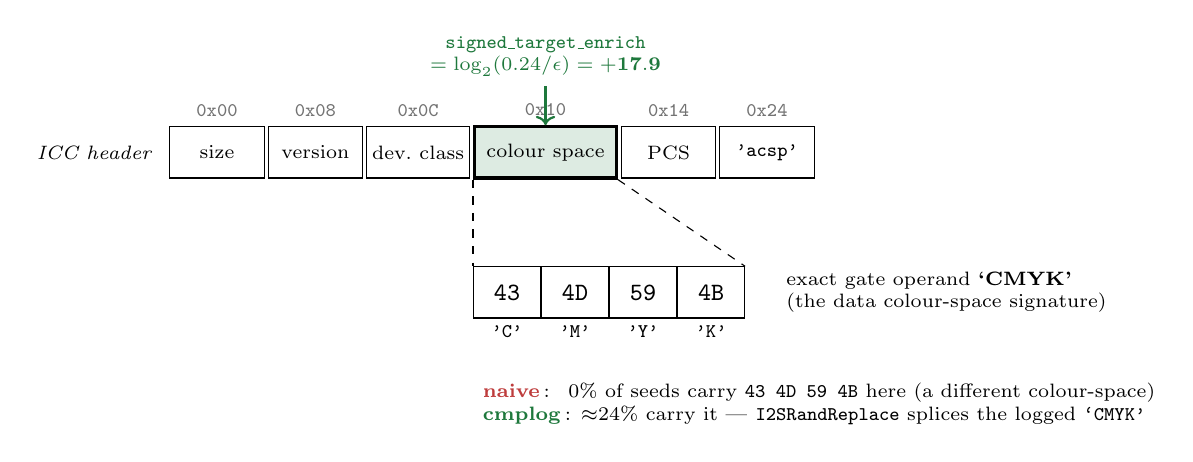
\begin{tikzpicture}[font=\footnotesize,
  fld/.style={draw,minimum height=6.5mm,minimum width=12mm,font=\scriptsize,inner sep=2pt},
  gate/.style={draw,very thick,fill=winc!15,minimum height=6.5mm,minimum width=18mm,font=\scriptsize},
  byte/.style={draw,minimum width=8.5mm,minimum height=6.5mm,font=\ttfamily\small},
  off/.style={font=\scriptsize\ttfamily,text=black!55}]
% --- ICC profile header: key fields at their real offsets ---
\node[fld] (size) {size};
\node[fld,right=1pt of size] (ver)  {version};
\node[fld,right=1pt of ver]  (dev)  {dev.\ class};
\node[gate,right=1pt of dev] (cs)   {colour space};
\node[fld,right=1pt of cs]   (pcs)  {PCS};
\node[fld,right=1pt of pcs]  (acsp) {\ttfamily 'acsp'};
\node[off,above=0pt of size]{0x00}; \node[off,above=0pt of ver]{0x08};
\node[off,above=0pt of dev]{0x0C};  \node[off,above=0pt of cs]{0x10};
\node[off,above=0pt of pcs]{0x14};  \node[off,above=0pt of acsp]{0x24};
\node[left=3pt of size,font=\scriptsize\itshape]{ICC header};
% --- enrichment callout on the gate field ---
\node[above=5mm of cs,font=\scriptsize,align=center,text=winc] (en)
     {\texttt{signed\_target\_enrich}\\$=\log_2(0.24/\epsilon)=\mathbf{+17.9}$};
\draw[->,winc,thick] (en) -- (cs.north);
% --- zoom the gate field into its 4 operand bytes ---
\node[byte,below=11mm of cs.south west,anchor=north west] (b0) {43};
\node[byte,right=0pt of b0] (b1) {4D};
\node[byte,right=0pt of b1] (b2) {59};
\node[byte,right=0pt of b2] (b3) {4B};
\node[font=\ttfamily\scriptsize,below=-1pt of b0]{'C'};
\node[font=\ttfamily\scriptsize,below=-1pt of b1]{'M'};
\node[font=\ttfamily\scriptsize,below=-1pt of b2]{'Y'};
\node[font=\ttfamily\scriptsize,below=-1pt of b3]{'K'};
\draw[dashed] (cs.south west) -- (b0.north west);
\draw[dashed] (cs.south east) -- (b3.north east);
\node[right=4mm of b3,align=left,font=\scriptsize]
     {exact gate operand \textbf{`CMYK'}\\(the data colour-space signature)};
% --- per-fuzzer frequency at this offset ---
\node[below=7mm of b0.south west,anchor=north west,align=left,font=\scriptsize] {%
  \textcolor{losc}{\textbf{naive}}\,:\ \ \,0\% of seeds carry \texttt{43 4D 59 4B} here (a different colour-space)\\
  \textcolor{winc}{\textbf{cmplog}}\,: $\approx$24\% carry it --- \texttt{I2SRandReplace} splices the logged \texttt{`CMYK'}};
\end{tikzpicture}\\[2pt]
{\footnotesize The gate operand of \texttt{lcms/2246} is the ICC \emph{data colour-space
signature} at offset \texttt{0x10}; \texttt{operand\_enrichment} measures how often each
fuzzer's corpus carries the exact bytes \emph{there}. Header field offsets are the ICC
format; the measured signal is \texttt{signed\_target\_enrich}$=+17.9$ (naive places the
literal in 0\% of its seeds), of which $\approx$24\% is the implied cmplog operand-offset rate.}
\end{center}

\paragraph{Sub-case: the literal \emph{floats} (no fixed offset).} Three of these
branches place the literal at a \emph{content-dependent} position rather than a
fixed file offset --- an XML entity name, a comment marker --- so the enrichment
test above cannot be anchored. The mechanism is identical (paste the exact
literal); only the operand's position differs, so we confirm them by the Layer-1
\mbox{cmplog\,$\succ$\,naive} advantage plus the \emph{absence} of any fixed-offset
signature (\texttt{gate\_signature == false}). Real example
(\texttt{libxml2}, \texttt{xmlGetPredefinedEntity}, \texttt{entities.c:307}):

\begin{lstlisting}[style=c]
switch (name[0]) {                       // name = a parsed entity reference
case 'a':                                // <-- blocker: needs the "amp"/"apos" name
    if (xmlStrEqual(name, "amp"))  return &xmlEntityAmp;
    if (xmlStrEqual(name, "apos")) return &xmlEntityApos;
    break;
default: return NULL;                    // naive lands here on all 479 of its calls
}
\end{lstlisting}
\noindent{\footnotesize cmplog takes \texttt{case 'a'} 63 times by splicing the
logged \texttt{"amp"}/\texttt{"apos"} operands into the input; naive never spells
them. The literal sits wherever the \texttt{\&\dots;} reference occurs, so there is
no fixed offset to measure --- hence the no-signature confirmation.}

\paragraph{Sub-case: confirmed by the value-distance route (6 branches).} Six
branches (5 curl, 1 harfbuzz; operands \texttt{"Host:"}, \texttt{"://"},
\texttt{"pop3"}, \texttt{"GPOS"}) are the \emph{same} exact-literal mechanism but
could not be anchored for the byte-frequency enrichment test, so the arbiter
confirmed them with \texttt{value\_distance\_reached} instead: the cmplog
(I2S) corpus lands the exact operand (residual~$0$) while the \emph{blind}
non-I2S corpus stalls at a positive Hamming residual. This is exactly category~1
--- ``paste the exact bytes'' --- measured by closure-of-distance rather than
enrichment (the same situation as the floating-offset sub-case above, where the
enrichment test also could not be anchored). Real example
(\texttt{curl/129}, \texttt{strncmp(line,\,"Host:",\,5)}): the I2S side closes the
whole \texttt{distance\_gap}$=0.8$ to the operand (\texttt{distance\_closure\_ratio}$=1.0$),
the blind side stalls $0.8$ away.

\metricbox{value\_distance\_reached}
{\texttt{distance\_gap} = how far the non-I2S corpus's nearest seed stalls from the target operand; \texttt{distance\_closure\_ratio} = fraction of that gap the I2S corpus closes ($1.0$ = lands it exactly)}
{winner\_closer == true AND distance\_gap > 0 AND distance\_closure\_ratio >= 0.5}
{curl/129, operand \texttt{"Host:"} --- \texttt{distance\_gap}$=0.8$, \texttt{distance\_closure\_ratio}$=1.0$: the I2S side lands the literal, the blind side never does. \emph{(Earlier split off as ``last-mile value precision''; folded into category~1, 2026-06-25 --- the rule compares I2S vs.\ \emph{naive}, i.e.\ plain literal substitution, not a distinct mechanism.)}}

\paragraph{Sub-case: the operand sits behind a multi-stage container (8 branches).}
Eight branches (\texttt{bloaty/87,90}, \texttt{harfbuzz/6236}, \texttt{lcms/2113},
\texttt{libpng/3820,3965}, \texttt{libxml2/6909,7287}) reach the gate only after
several \emph{interlocking} fields validate --- an ELF section table, a PNG chunk
grammar, an XML scheme$+$attribute. We initially split these off as ``structural
assembly depth,'' but the move is still the \emph{same} one: I2S pastes the exact
field literal(s); there are simply \emph{several} operands scattered across a
multi-stage container rather than one. ``Multi-operand'' is a \emph{description},
not a separate mechanism --- and crucially \emph{no cheap signal distinguishes it
from single-operand category~1}. The original \texttt{depth\_reach} metric
(\texttt{depth\_lift}~$=$ winner/loser per-seed executions of the blocker line) is
\emph{loop-confounded} --- \texttt{bloaty/90}'s ``blocker'' is literally
\texttt{for (\ldots; i < elf.section\_count(); i++)}, so the $2375\times$ ``depth''
is just loop trips, not assembly --- and \emph{near-tautological} (it runs the
already-arriving resolving/blocking seeds). Byte-offset enrichment cannot anchor
(the fields float, $5/8$ have \texttt{gate\_signature == false}); an in-function
magic-gate count does not separate them from category~1 (the interlocking checks
live in \emph{callee} functions). So they fold into category~1, confirmed --- like
the floating-offset sub-case --- by the Layer-1 \mbox{cmplog\,$\succ$\,naive}
advantage. \emph{(Folded 2026-06-25.)}

% =====================================================================
\section*{2.\ \ Exact number / enum gate \hfill {\normalsize\texttt{i2s\_numeric\_tag\_substitution} ($n=39$)}}
Same move, but the thing matched is a small \emph{number} --- a version code, an
enum, a \texttt{switch}-case selector --- not a string. I2S substitutes the
precise value. We split it from category~1 only because ``it's a number'' vs
``it's a string'' matters when you later try to \emph{recognize} the gate; the
mechanism (paste the exact value) is identical.

\begin{lstlisting}[style=c]
// version/enum dispatch -- gate needs one exact constant
switch (header.version) {
  case 2:  parse_v2(...); break;    // <-- blocker: only the value 2 reaches it
  default: reject();
}
\end{lstlisting}

\noindent\textbf{How we know.} The cmplog corpus over-represents the \emph{target}
constant and \emph{under}-represents the competing ``decoy'' values, exactly as
deterministic substitution of one logged operand would predict.

\metricbox{operand\_enrichment}
{\texttt{signed\_target\_enrich} (target value, $\log_2$ ratio) and \texttt{decoy\_enrich} (the competing value)}
{signed\_target\_enrich >= 1.0 AND decoy\_enrich <= 0.0}
{bloaty/34, switch-case constant --- \texttt{signed\_target\_enrich}$=11.2$ (target piled up) while \texttt{decoy\_enrich}$=-3.7$ (wrong values drained).}

\begin{center}
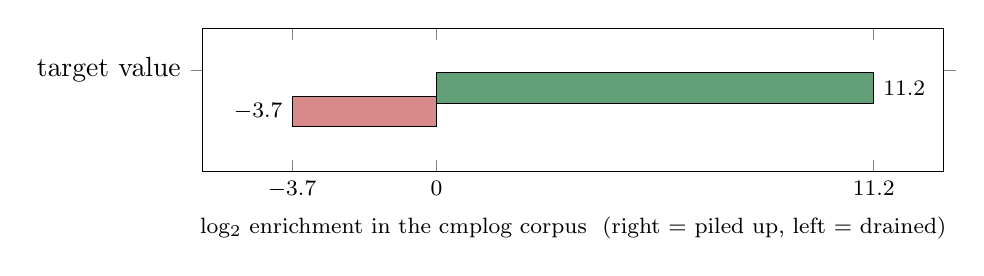
\begin{tikzpicture}
\begin{axis}[
  width=11cm, height=3.4cm, xbar, xmin=-6, xmax=13,
  bar width=11pt, enlarge y limits=0.7,
  symbolic y coords={decoy value, target value},
  ytick=data, xtick={-3.7,0,11.2}, xticklabel style={font=\footnotesize},
  nodes near coords, every node near coord/.append style={font=\footnotesize},
  xlabel={\footnotesize log$_2$ enrichment in the cmplog corpus \ (right = piled up, left = drained)},
]
\addplot[fill=winc!70] coordinates {(11.2,target value)};
\addplot[fill=losc!60] coordinates {(-3.7,decoy value)};
\end{axis}
\end{tikzpicture}\\[-2pt]
{\footnotesize I2S concentrates the corpus on the one right number and steers it away from the wrong ones.}
\end{center}

% =====================================================================
\section*{At a glance}
\begin{center}\small
\begin{tabular}{@{}p{3.6cm}clp{5.0cm}@{}}
\toprule
\textbf{Category} & \textbf{$n$} & \textbf{Tool / metric} & \textbf{One-line reason} \\
\midrule
string / literal gate & 199 & operand\_enrichment / \texttt{signed\_target\_enrich} & paste the exact bytes (incl.\ 3 floating-offset \texttt{gate\_signature}=false, 6 value-distance-route, 8 multi-stage container) \\
numeric / enum gate & 39 & operand\_enrichment / \texttt{signed\_target\_enrich}+\texttt{decoy\_enrich} & paste the exact number \\
\midrule
\textbf{I2S-pro total} & \textbf{238} & & \\
\bottomrule
\end{tabular}
\end{center}

\noindent\footnotesize Counts and example metrics regenerated from
\texttt{bench/dataset.jsonl}; verify rules are the deterministic arbiter rules
(no LLM in the decision).
\end{document}
